\chapter{बहुलक}\label{ch:g12:polymers}

फ़्लीस जैकेट पिघली हुई पेय-बोतलों से काती जा सकती है; पर्वतारोहण की रस्सी
नायलॉन की बनी होती है; यह पृष्ठ सेलुलोज़ है, जिसे पेड़ों ने बनाया है। तीनों
\omterm{def:g12:polymers:polymer}{बहुलक} हैं: हज़ारों \omterm{def:g7:atoms-and-molecules:atom}{परमाणु} लंबे \omterm{def:g7:atoms-and-molecules:molecule}{अणु}, जो एक छोटी
इकाई को बार-बार दोहराकर बने हैं। उनके गुण --- नरम या कठोर, प्रत्यास्थ या
भंगुर, पिघलने योग्य या नहीं --- उनमें मौजूद \omterm{def:g7:atoms-and-molecules:atom}{परमाणुओं} से कम, और
उनकी लंबी श्रृंखलाओं की व्यवस्था से अधिक आते हैं।

\begin{recall}
\omterm{def:g8:plastics:plastic}{प्लास्टिक} बहुत लंबे \omterm{def:g7:atoms-and-molecules:molecule}{अणुओं} से बने होते हैं; \omterm{def:g8:plastics:thermoplastic}{थर्मोप्लास्टिक} गरम करने पर
नरम पड़ते हैं, \omterm{def:g8:plastics:thermoplastic}{थर्मोसेट} नहीं (\cref{ch:g8:plastics})। \omterm{def:g11:functional-groups:alcohol}{ऐल्कोहॉल}, अम्ल, \omterm{def:g11:functional-groups:carboxylic-acid}{एस्टर},
\omterm{def:g11:functional-groups:amine}{ऐमीन} और \omterm{def:g11:functional-groups:amine}{ऐमाइड} समूह (\cref{ch:g11:functional-groups})। \omterm{def:g12:curly-arrows:categories}{योगज अभिक्रिया}
बिना कोई \omterm{def:g7:atoms-and-molecules:atom}{परमाणु} खोए दो \omterm{def:g7:atoms-and-molecules:molecule}{अणुओं} को एक में जोड़ती है
(\cref{ch:g12:curly-arrows})।
\end{recall}

\begin{omfigure}
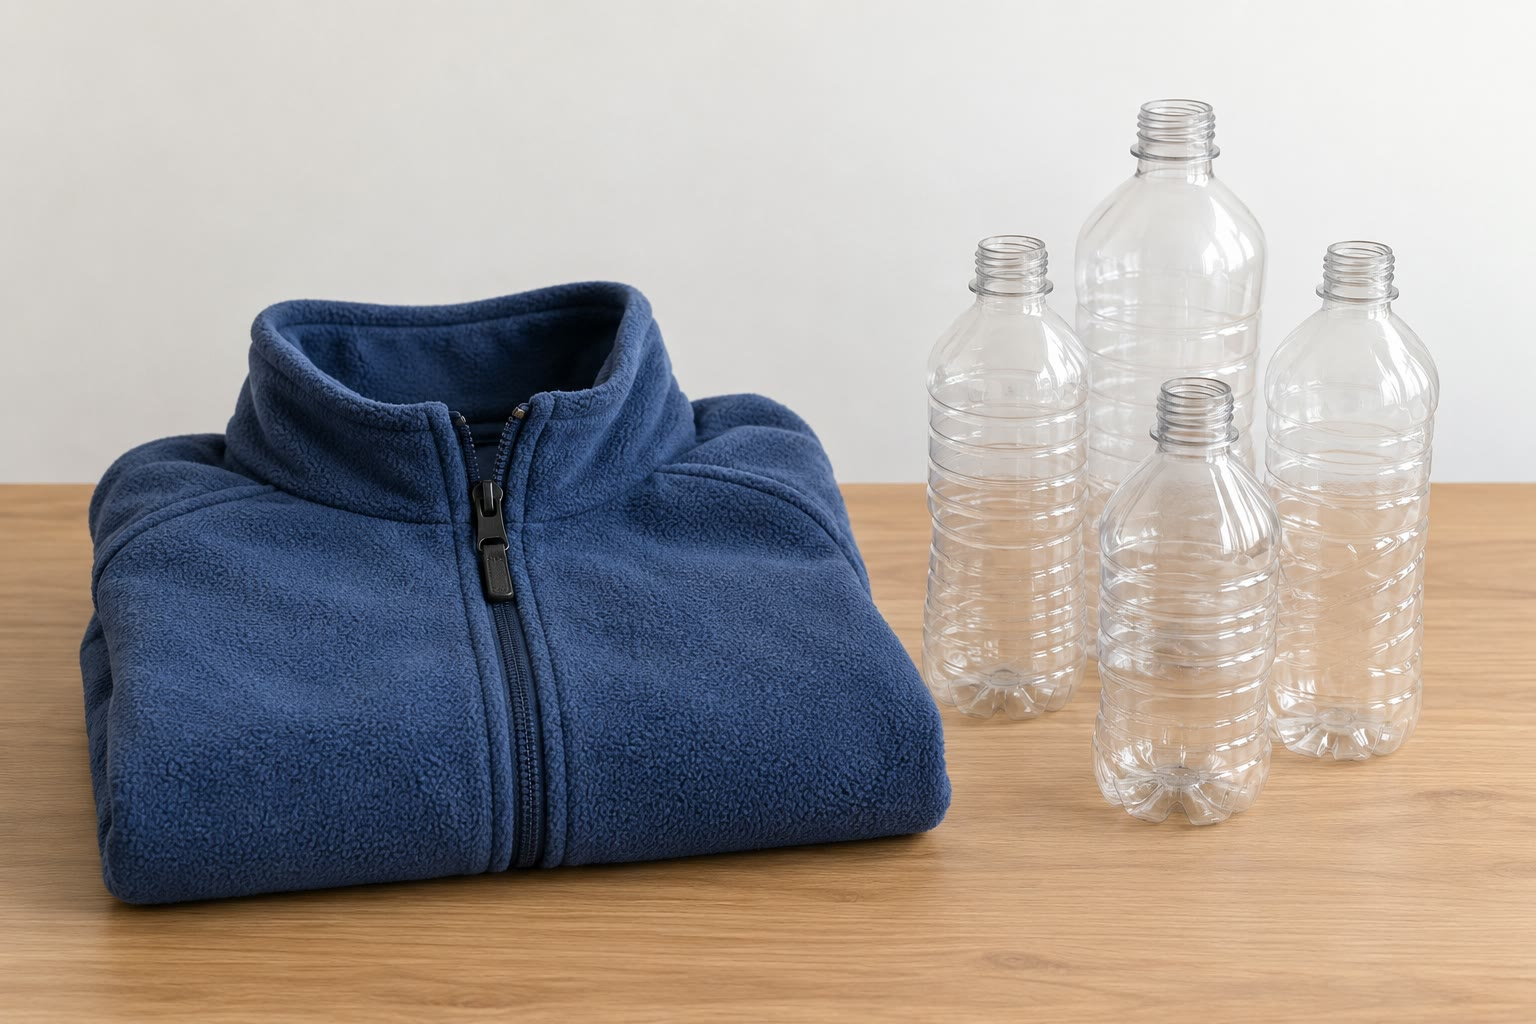
\includegraphics[width=0.45\linewidth]{images/book1/ai/g12-fleece-bottles.jpg}

{\small इस्तेमाल की हुई पेय-बोतलें और एक फ़्लीस जैकेट: वही \omterm{def:g12:polymers:polymer}{बहुलक}, दो
रूपों में।}
\end{omfigure}

\section{एकलक, बहुलक, पुनरावृत्त इकाइयाँ}

\begin{definition}[बहुलक, एकलक, बहुलकीकरण]\label{def:g12:polymers:polymer}
\emph{बहुलक}\index{बहुलक} बहुत बड़े \omterm{def:g7:atoms-and-molecules:molecule}{अणुओं}, बृहदणुओं, से बना एक पदार्थ है,
जिनमें से हर एक अनेक छोटी इकाइयों से बना है जो एक के बाद एक आबंधित
होती हैं। जिन छोटे \omterm{def:g7:atoms-and-molecules:molecule}{अणुओं} से वह बनता है, वे उसके
\emph{एकलक}\index{एकलक} हैं; उन्हें जोड़ने वाली अभिक्रिया
\emph{बहुलकीकरण}\index{बहुलकीकरण} है।
\end{definition}

\begin{definition}[पुनरावृत्त इकाई, बहुलकीकरण की कोटि]\label{def:g12:polymers:repeat-unit}
किसी \omterm{def:g12:polymers:polymer}{बहुलक} की \emph{पुनरावृत्त इकाई}\index{पुनरावृत्त इकाई} \omterm{def:g7:atoms-and-molecules:atom}{परमाणुओं} का वह सबसे छोटा
समूह है जिसकी पुनरावृत्ति से श्रृंखला बनती है; उसे एक सूचकांक $n$ के साथ
कोष्ठकों के बीच लिखा जाता है। किसी श्रृंखला में पुनरावृत्त इकाइयों की संख्या $n$
उसकी \emph{बहुलकीकरण की कोटि}\index{बहुलकीकरण की कोटि} है।
\end{definition}

\begin{omfigure}
\[
  n\;\ce{CH2=CH2}
  \quad\longrightarrow\quad
  \chemfig{-[@{op1,.75}]CH_2-CH_2-[@{cl1,0.25}]}
  \polymerdelim[height=6pt, depth=6pt, indice=n]{op1}{cl1}
\]

{\small एथीन का \omterm{def:g12:polymers:polymer}{बहुलकीकरण}: \omterm{def:g12:polymers:polymer}{एकलक} के $n$ \omterm{def:g7:atoms-and-molecules:molecule}{अणु} पॉलीएथीन की एक
श्रृंखला देते हैं, जिसकी \omterm{def:g12:polymers:repeat-unit}{पुनरावृत्त इकाई} \ce{-CH2-CH2-} कोष्ठकों के बीच
लिखी जाती है।}
\end{omfigure}

\begin{proposition}[बहुलक का मोलर द्रव्यमान]\label{prop:g12:polymers:molar-mass}
\omterm{def:g12:polymers:repeat-unit}{बहुलकीकरण की कोटि} $n$ वाली श्रृंखला का \omterm{def:g10:the-mole:molar-mass}{मोलर द्रव्यमान} है
\[
  M(\text{बहुलक}) \approx n \times M(\text{पुनरावृत्त इकाई}) ,
\]
क्योंकि बड़े $n$ के लिए श्रृंखला के दोनों सिरे नगण्य हैं।
\end{proposition}

\begin{proof}
श्रृंखला $n$ पुनरावृत्त इकाइयाँ और कुछ-कुछ \omterm{def:g7:atoms-and-molecules:atom}{परमाणुओं} वाले दो अंत्य समूह है;
हज़ारों में $n$ के लिए, अंत्य समूह पूरे के एक हज़ारवें भाग से भी
कम भारी होते हैं।
\end{proof}

\begin{example}[एक पॉलीएथीन श्रृंखला]\label{ex:g12:polymers:pe}
% ledger: aw:C, aw:H
जिस पॉलीएथीन श्रृंखला का \omterm{def:g10:the-mole:molar-mass}{मोलर द्रव्यमान} \qty{280000}{g/mol} हो, उसमें
$n = 280000/28.0 = 10000$ पुनरावृत्त इकाइयाँ हैं, यानी एक पंक्ति में बीस हज़ार कार्बन \omterm{def:g7:atoms-and-molecules:atom}{परमाणु}।
किसी वास्तविक नमूने में सभी श्रृंखलाओं की लंबाई समान नहीं होती:
$n$ एक औसत है।
\end{example}

\section{योगज बहुलक}

\begin{definition}[योगज बहुलक, संघनन बहुलक]\label{def:g12:polymers:addition-polymer}
\emph{योगज बहुलक}\index{योगज बहुलक} \ce{C=C} \omterm{def:g10:lewis-and-shape:multiple-bond}{द्विआबंध} वाले \omterm{def:g12:polymers:polymer}{एकलकों} के
योग से बनता है, बिना किसी अन्य उत्पाद के: उसकी
\omterm{def:g12:polymers:repeat-unit}{पुनरावृत्त इकाई} में वही \omterm{def:g7:atoms-and-molecules:atom}{परमाणु} होते हैं जो \omterm{def:g12:polymers:polymer}{एकलक} में। \emph{संघनन
बहुलक}\index{संघनन बहुलक} दो \omterm{def:g11:functional-groups:functional-group}{क्रियात्मक समूहों} के बीच ऐसी अभिक्रियाओं से बनता है
जो दो \omterm{def:g12:polymers:polymer}{एकलकों} को जोड़ती हैं और हर कड़ी पर एक छोटा \omterm{def:g7:atoms-and-molecules:molecule}{अणु}, आम तौर पर पानी,
मुक्त करती हैं।
\end{definition}

\begin{omfigure}
\footnotesize
\renewcommand{\arraystretch}{1.5}
\begin{tabular}{l l l l}
\hline
\omterm{def:g12:polymers:polymer}{एकलक} & \omterm{def:g12:polymers:polymer}{बहुलक} & \omterm{def:g12:polymers:repeat-unit}{पुनरावृत्त इकाई} & उपयोग \\
\hline
एथीन \ce{CH2=CH2} & पॉलीएथीन (PE) & \ce{-CH2-CH2-} & थैले, बोतलें \\
क्लोरोएथीन \ce{CH2=CHCl} & पॉली(विनाइल क्लोराइड) (PVC) & \ce{-CH2-CHCl-} & पाइप, चौखटें \\
फ़ेनिलएथीन \ce{CH2=CH-C6H5} & पॉलीस्टाइरीन (PS) & \ce{-CH2-CH(C6H5)-} & कप, फ़ोम \\
टेट्राफ़्लुओरोएथीन \ce{CF2=CF2} & PTFE & \ce{-CF2-CF2-} & नॉन-स्टिक बर्तन \\
\hline
\end{tabular}\par\medskip

{\small चार \omterm{def:g12:polymers:addition-polymer}{योगज बहुलक}। हर एक में \omterm{def:g12:polymers:polymer}{एकलक} का \omterm{def:g10:lewis-and-shape:multiple-bond}{द्विआबंध}
खुलता है, और उसके दोनों कार्बन श्रृंखला से जुड़ जाते हैं।}
\end{omfigure}

\begin{method}[बहुलक से एकलक ज्ञात करना]\label{met:g12:polymers:monomer}
\begin{enumerate}
  \item \omterm{def:g12:polymers:repeat-unit}{पुनरावृत्त इकाई} खोजिए: वह सबसे छोटा समूह जिसकी पुनरावृत्ति से
        श्रृंखला बनती है।
  \item यदि मुख्य श्रृंखला में केवल कार्बन \omterm{def:g7:atoms-and-molecules:atom}{परमाणु} हैं, तो यह \omterm{def:g12:polymers:addition-polymer}{योगज
        बहुलक} है: \omterm{def:g12:polymers:repeat-unit}{पुनरावृत्त इकाई} की मुख्य श्रृंखला के दोनों कार्बनों के बीच
        \omterm{def:g10:lewis-and-shape:multiple-bond}{द्विआबंध} वापस रखिए। यही \omterm{def:g12:polymers:polymer}{एकलक} है।
  \item यदि मुख्य श्रृंखला में \omterm{def:g11:functional-groups:carboxylic-acid}{एस्टर} या \omterm{def:g11:functional-groups:amine}{ऐमाइड} कड़ियाँ हैं, तो यह
        \omterm{def:g12:polymers:addition-polymer}{संघनन बहुलक} है: हर कड़ी काटिए, और हर पक्ष को
        मुक्त हुए छोटे \omterm{def:g7:atoms-and-molecules:molecule}{अणु} के \omterm{def:g7:atoms-and-molecules:atom}{परमाणु} लौटाइए (\ce{-OH} को
        \ce{C=O} की ओर, \ce{-H} को \ce{O} या \ce{N} की ओर)। वही
        \omterm{def:g12:polymers:polymer}{एकलक} हैं।
\end{enumerate}
\end{method}

\begin{example}[PVC का एकलक]\label{ex:g12:polymers:pvc}
श्रृंखला \ce{-CH2-CHCl-CH2-CHCl-CH2-CHCl-} \ce{-CH2-CHCl-} को दोहराती है; उसकी
मुख्य श्रृंखला में केवल कार्बन हैं, इसलिए \omterm{def:g12:polymers:polymer}{एकलक}
\ce{CH2=CHCl}, क्लोरोएथीन, है।
\end{example}

\section{संघनन बहुलक}

एक क्रियाशील समूह वाला \omterm{def:g12:polymers:polymer}{एकलक} केवल एक बार आबंध बना सकता है: वह श्रृंखला को समाप्त कर देता है।
संघनन से श्रृंखला बनाने के लिए हर \omterm{def:g12:polymers:polymer}{एकलक} को दो समूह चाहिए, हर
सिरे पर एक।

\begin{example}[PET, एक पॉलिएस्टर]\label{ex:g12:polymers:pet}
% ledger: aw:C, aw:H, aw:O
एथेन-1,2-डाइऑल, \ce{HO-CH2-CH2-OH}, में दो \omterm{def:g11:functional-groups:alcohol}{ऐल्कोहॉल} समूह हैं;
बेंज़ीन-1,4-डाइकार्बोक्सिलिक अम्ल, \ce{HOOC-C6H4-COOH}, में दो अम्ल समूह। हर
अम्ल समूह एक \omterm{def:g11:functional-groups:alcohol}{ऐल्कोहॉल} समूह के साथ \omterm{def:g11:functional-groups:carboxylic-acid}{एस्टर} बनाता है और पानी मुक्त करता है:
श्रृंखला दोनों सिरों से बढ़ती है। \omterm{def:g12:polymers:polymer}{बहुलक} पॉली(एथिलीन टेरेफ़्थेलेट),
PET, है, जो पेय-बोतलों और पॉलिएस्टर रेशों का पदार्थ है। उसकी \omterm{def:g12:polymers:repeat-unit}{पुनरावृत्त
इकाई}, \ce{C10H8O4}, का \omterm{def:g10:the-mole:molar-mass}{मोलर द्रव्यमान} \qty{192.0}{g/mol} है, अर्थात
दोनों \omterm{def:g12:polymers:polymer}{एकलक} ($62.0 + 166.0$) घटा पानी के दो \omterm{def:g7:atoms-and-molecules:molecule}{अणु} ($36.0$)।
\end{example}

\begin{omfigure}
\setchemfig{atom sep=1.9em}
\chemfig{HO-CH_2-CH_2-OH}
\quad $+$ \quad
\chemfig{HO-C(=[2]O)-*6(-=-(-C(=[2]O)-OH)=-=)}

\medskip
$\longrightarrow$\quad
\chemfig{-[@{op2,.75}]O-CH_2-CH_2-O-C(=[2]O)-*6(-=-(-C(=[2]O)-[@{cl2,0.25}])=-=)}
\polymerdelim[height=20pt, depth=6pt, indice=n]{op2}{cl2}
\quad $+\ 2n\ \ce{H2O}$

{\small अपने दो \omterm{def:g12:polymers:polymer}{एकलकों} से PET: हर \omterm{def:g11:functional-groups:carboxylic-acid}{एस्टर} कड़ी (\ce{-CO-O-}
समूह) पानी का एक \omterm{def:g7:atoms-and-molecules:molecule}{अणु} मुक्त करती है।}
\end{omfigure}

\begin{example}[नायलॉन-6,6, एक पॉलिऐमाइड]\label{ex:g12:polymers:nylon}
हेक्सेन-1,6-डाइऐमीन, \ce{H2N-(CH2)6-NH2}, और हेक्सेनडाइओइक अम्ल,
\ce{HOOC-(CH2)4-COOH}, \omterm{def:g11:functional-groups:amine}{ऐमाइड} कड़ियों से जुड़ते हैं, जिनमें से हर एक पानी का एक
\omterm{def:g7:atoms-and-molecules:molecule}{अणु} मुक्त करती है:
\[
  \cdots\ce{-NH-(CH2)6-NH-CO-(CH2)4-CO-}\cdots
\]
नाम में दोनों छक्के हर \omterm{def:g12:polymers:polymer}{एकलक} के कार्बन \omterm{def:g7:atoms-and-molecules:atom}{परमाणु} गिनते हैं।
पड़ोसी श्रृंखलाओं की \omterm{def:g11:functional-groups:amine}{ऐमाइड} कड़ियाँ \omterm{def:g11:polarity-and-cohesion:hydrogen-bond}{हाइड्रोजन आबंधों} द्वारा एक-दूसरे को आकर्षित करती हैं,
जिससे नायलॉन के रेशे मज़बूत होते हैं।
\end{example}

\begin{history}[कैरोथर्स और नायलॉन]
% ledger: hist:polyamides-1934, hist:nylon-production-1939
रसायनज्ञ वॉलेस कैरोथर्स, जो एक रसायन कंपनी की एक अनुसंधान प्रयोगशाला के
प्रमुख थे, यह सिद्ध करने निकले कि \omterm{def:g12:polymers:polymer}{बहुलक} वास्तव में विशाल
\omterm{def:g7:atoms-and-molecules:molecule}{अणु} हैं और उन्हें जान-बूझकर बनाया जा सकता है। उनकी टीम ने पहले पॉलिएस्टर बनाए,
जो उपयोगी होने के लिए बहुत आसानी से पिघल जाते थे; 1934 में वे \omterm{def:g11:functional-groups:amine}{ऐमीनों} की ओर मुड़े और
पॉलिऐमाइड बनाए, जिनमें वह रेशा भी था जिसे बाद में नायलॉन नाम मिला। नायलॉन का
उत्पादन 1939 में शुरू हुआ, पहले मोज़ों के रूप में जिन्होंने एक
विश्व मेले में सनसनी फैला दी, फिर पैराशूट, रस्सियों और टूथब्रश के रेशों के रूप में।
\end{history}

\begin{omfigure}
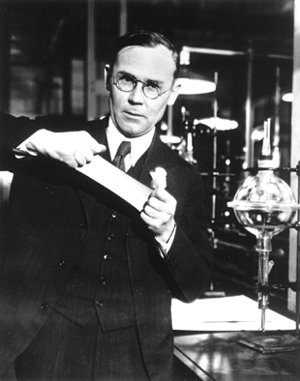
\includegraphics[width=0.24\linewidth]{images/book1/carothers.jpg}

{\small अपनी प्रयोगशाला में वॉलेस कैरोथर्स।}
\end{omfigure}

\section{संरचना और गुण}

एक ही \omterm{def:g12:polymers:polymer}{बहुलक} के दो नमूने बहुत अलग व्यवहार कर सकते हैं: मायने यह रखता है कि
श्रृंखलाएँ कितनी लंबी हैं, उनकी आकृति कैसी है, और वे कैसे सजी हैं।

\begin{proposition}[श्रृंखलाएँ और गुण]\label{prop:g12:polymers:properties}
\begin{itemize}
  \item लंबी श्रृंखलाएँ अधिक उलझती हैं: पदार्थ अधिक मज़बूत होता है और
        ऊँचे ताप पर पिघलता है।
  \item रैखिक श्रृंखलाएँ व्यवस्थित, \emph{क्रिस्टलीय} क्षेत्रों में अगल-बगल
        सज सकती हैं; शाखित श्रृंखलाएँ नहीं सज सकतीं, और
        अव्यवस्थित, \emph{अक्रिस्टलीय}, रहती हैं। क्रिस्टलीय क्षेत्र
        \omterm{def:g12:polymers:polymer}{बहुलक} को अधिक घना, अधिक कठोर और कम पारदर्शी बनाते हैं।
  \item केवल अंतराआण्विक बलों से अगल-बगल टिकी श्रृंखलाएँ गरम करने पर
        एक-दूसरे पर फिसलती हैं: \omterm{def:g12:polymers:polymer}{बहुलक} \omterm{def:g8:plastics:thermoplastic}{थर्मोप्लास्टिक} है। सहसंयोजी
        \emph{तिर्यक-बंधों} से जुड़ी श्रृंखलाएँ नहीं फिसल सकतीं: \omterm{def:g12:polymers:polymer}{बहुलक}
        \omterm{def:g8:plastics:thermoplastic}{थर्मोसेट} है, या, कम तिर्यक-बंधों के साथ, रबड़ जैसा प्रत्यास्थ
        ठोस।
\end{itemize}
\end{proposition}

\begin{proof}
गरम करने से श्रृंखलाओं को उनके बीच के अंतराआण्विक
बलों (\cref{ch:g11:polarity-and-cohesion}) पर विजय पाने लायक ऊर्जा मिलती है, जो
\omterm{def:g10:lewis-and-shape:covalent-bond}{सहसंयोजी आबंधों} से दुर्बल हैं; श्रृंखलाओं के बीच जितना अधिक संपर्क, उतनी ही
अधिक ऊर्जा लगती है। तिर्यक-बंध सहसंयोजी हैं: उन्हें तोड़ने से
पदार्थ पिघलने के बजाय नष्ट हो जाता है।
\end{proof}

\begin{omfigure}
\begin{tikzpicture}[font=\footnotesize, line width=1pt, line cap=round,
    lab/.style={below, align=center, text width=2.8cm}]
  % linear, packed (crystalline)
  \begin{scope}
    \foreach \y in {0,0.25,0.5,0.75,1.0}
      \draw[omDef] plot[smooth, domain=0:2.2, samples=25] (\x, {\y + 0.05*sin(400*\x)});
    \node[lab] at (1.1,-0.2) {रैखिक श्रृंखलाएँ\\ सीधी सजी: क्रिस्टलीय};
  \end{scope}
  % linear, tangled (amorphous)
  \begin{scope}[xshift=3.4cm]
    \draw[omDef] plot[smooth] coordinates {(0,0.2) (0.5,0.9) (1.0,0.3) (1.4,1.1) (2.0,0.5) (2.2,0.9)};
    \draw[omProp] plot[smooth] coordinates {(0,0.9) (0.4,0.3) (0.9,1.0) (1.5,0.2) (1.9,1.0) (2.2,0.3)};
    \draw[black!60] plot[smooth] coordinates {(0.1,0.55) (0.7,0.1) (1.2,0.75) (1.7,0.55) (2.2,0.1)};
    \node[lab] at (1.1,-0.2) {रैखिक श्रृंखलाएँ\\ उलझी: अक्रिस्टलीय};
  \end{scope}
  % branched
  \begin{scope}[xshift=6.8cm]
    \draw[omDef] plot[smooth] coordinates {(0,0.5) (0.6,0.6) (1.2,0.45) (1.8,0.65) (2.2,0.5)};
    \draw[omDef] (0.5,0.6) -- (0.35,1.05) (1.0,0.5) -- (1.15,0.05) (1.6,0.6) -- (1.5,1.1) (1.6,0.6) -- (1.95,1.0);
    \node[lab] at (1.1,-0.2) {शाखित श्रृंखलाएँ:\\ सज नहीं सकतीं};
  \end{scope}
  % cross-linked
  \begin{scope}[xshift=10.2cm]
    \foreach \y in {0.1,0.55,1.0}
      \draw[omDef] plot[smooth, domain=0:2.2, samples=25] (\x, {\y + 0.06*sin(300*\x)});
    \foreach \x/\a/\b in {0.4/0.1/0.55, 1.3/0.1/0.55, 0.9/0.55/1.0, 1.9/0.55/1.0}
      \draw[omProp, line width=1.6pt] (\x,\a) -- (\x,\b);
    \node[lab] at (1.1,-0.2) {तिर्यक-बंधित श्रृंखलाएँ:\\ पिघलती नहीं};
  \end{scope}
\end{tikzpicture}

{\small \omterm{def:g12:polymers:polymer}{बहुलक} श्रृंखलाओं की चार व्यवस्थाएँ। तिर्यक-बंध (नारंगी)
श्रृंखलाओं के बीच \omterm{def:g10:lewis-and-shape:covalent-bond}{सहसंयोजी आबंध} हैं।}
\end{omfigure}

\begin{example}[दो पॉलीएथीन]\label{ex:g12:polymers:two-pe}
बहुत ऊँचे दाब पर बनी पॉलीएथीन में बहुत-सी छोटी शाखाएँ होती हैं: उसकी
श्रृंखलाएँ ठीक से नहीं सजतीं, और वह थैलों के लिए नरम, पारदर्शी फ़िल्में देती है। कम दाब पर
\omterm{def:g12:catalysis:catalyst}{उत्प्रेरक} के साथ बनाने पर उसकी श्रृंखलाएँ लगभग रैखिक होती हैं और
क्रिस्टलीय क्षेत्रों में सजती हैं: वह अधिक घनी और कठोर होती है, और दूध की
बोतलें और क्रेट देती है। वही \omterm{def:g12:polymers:polymer}{एकलक}, वही \omterm{def:g12:polymers:repeat-unit}{पुनरावृत्त इकाई}, भिन्न
वास्तु।
\end{example}

\section{प्राकृतिक बहुलक}

सजीव रसायनज्ञों से बहुत पहले से \omterm{def:g12:polymers:polymer}{बहुलक} बनाते आए हैं।

\begin{itemize}
  \item \textbf{सेलुलोज़} और \textbf{स्टार्च} दोनों ग्लूकोज़
        इकाइयों की श्रृंखलाएँ हैं, प्रति इकाई \ce{C6H10O5}, जो अलग-अलग ढंग से जुड़ी हैं: सेलुलोज़
        सीधे, मज़बूत रेशे बनाता है (लकड़ी, कपास, कागज़); स्टार्च
        कुंडलियाँ बनाता है जिन्हें शरीर पचा लेता है।
  \item \textbf{प्रोटीन} \omterm{def:g11:functional-groups:amine}{ऐमाइड} कड़ियों से जुड़े ऐमीनो अम्लों की श्रृंखलाएँ हैं,
        जो \cref{ch:g12:synthesis-strategy} के डाइपेप्टाइड वाले
        पेप्टाइड आबंध हैं।
  \item \textbf{डीएनए} न्यूक्लियोटाइडों की एक श्रृंखला है; उसकी चार
        प्रकार की इकाइयों का क्रम आनुवंशिक सूचना संचित करता है।
  \item \textbf{प्राकृतिक रबड़} आइसोप्रीन,
        \ce{CH2=C(CH3)-CH=CH2}, का एक \omterm{def:g12:polymers:addition-polymer}{योगज बहुलक} है, जिसे रबड़ के पेड़ की छाल से
        दूधिया द्रव, लेटेक्स, के रूप में एकत्र किया जाता है। सल्फ़र के साथ गरम करने पर उसकी श्रृंखलाएँ
        सल्फ़र सेतुओं से जुड़ जाती हैं: रबड़ अधिक सख़्त हो जाता है और अपनी
        आकृति बनाए रखता है, जैसे टायर में।
\end{itemize}

\begin{omfigure}
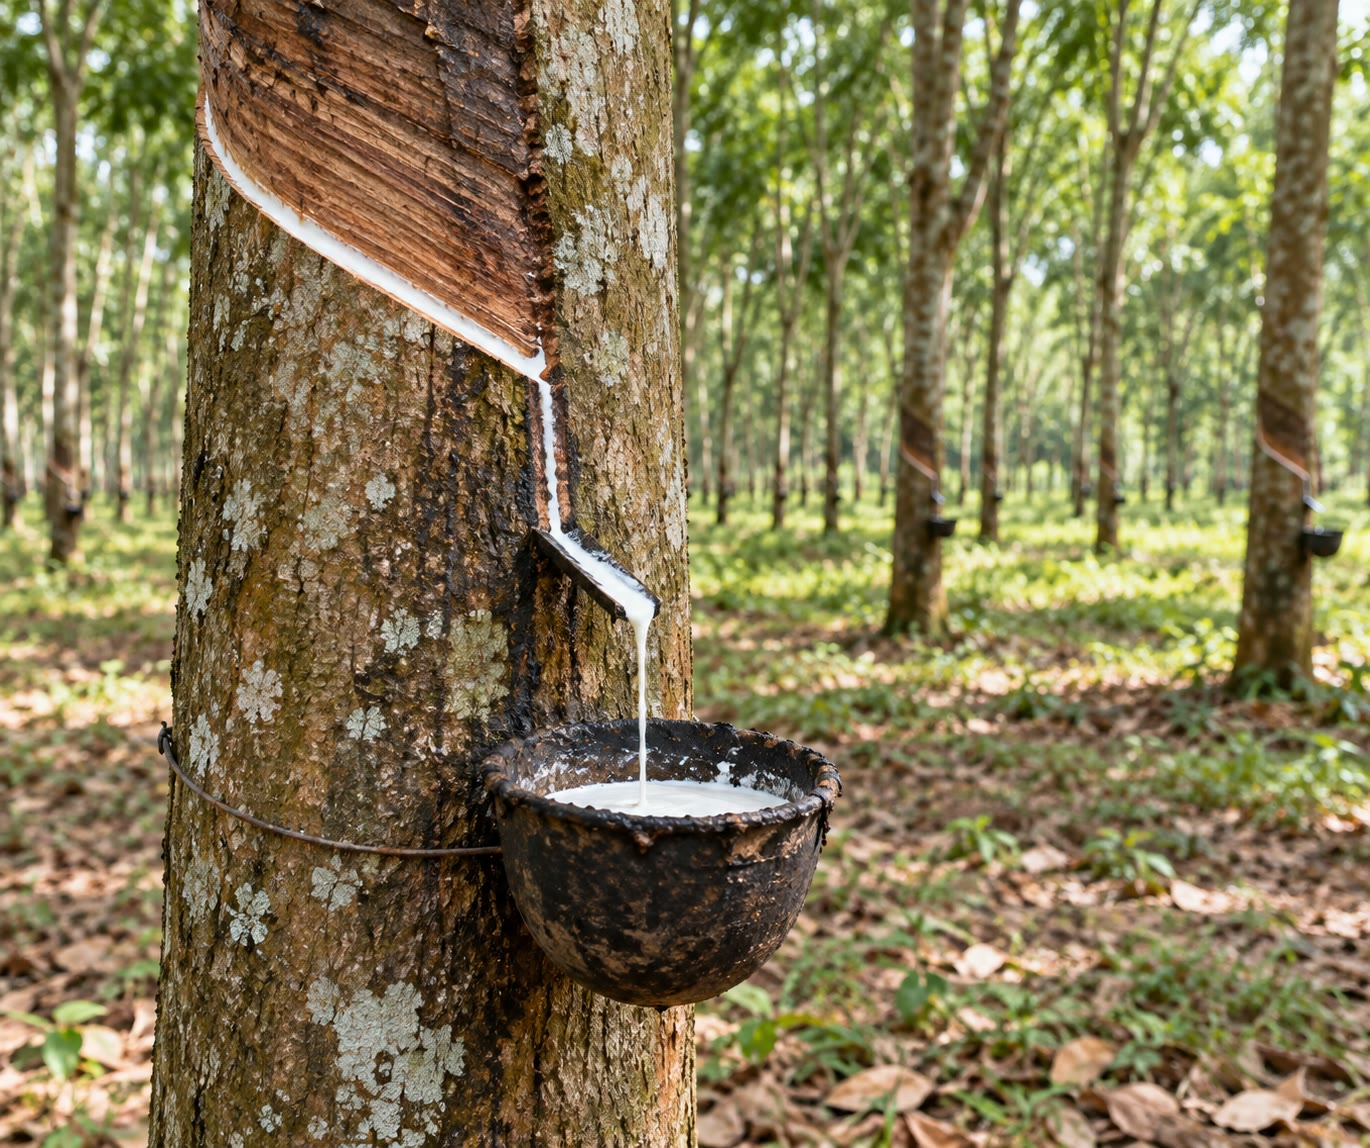
\includegraphics[width=0.45\linewidth]{images/book1/ai/g12-rubber-tapping.jpg}

{\small रबड़ के पेड़ से रस निकालना: छाल के एक चीरे से लेटेक्स बहकर एक
प्याले में जाता है।}
\end{omfigure}

\begin{remark}[बनाना और बिगाड़ना]\label{rem:g12:polymers:recycling}
\omterm{def:g8:plastics:thermoplastic}{थर्मोप्लास्टिक} को पिघलाकर फिर से आकार दिया जा सकता है: यांत्रिक \omterm{def:g5:raw-materials-and-recycling:recycling}{पुनर्चक्रण}।
\omterm{def:g12:polymers:addition-polymer}{संघनन बहुलक} को उलटी अभिक्रिया, जल-अपघटन, द्वारा
उसके \omterm{def:g12:polymers:polymer}{एकलकों} में भी तोड़ा जा सकता है, और \omterm{def:g12:polymers:polymer}{एकलकों} से नया \omterm{def:g12:polymers:polymer}{बहुलक} बनाया जा सकता है:
रासायनिक \omterm{def:g5:raw-materials-and-recycling:recycling}{पुनर्चक्रण}। \omterm{def:g8:plastics:thermoplastic}{थर्मोसेट} इनमें से कोई भी आसानी से नहीं कर सकता।
\end{remark}

\section{अभ्यास}

\begin{exercise}[$\star$]\label{exo:g12:polymers:1}
पॉलीप्रोपीन का \omterm{def:g12:polymers:polymer}{एकलक} बताइए, जिसकी \omterm{def:g12:polymers:repeat-unit}{पुनरावृत्त इकाई}
\ce{-CH2-CH(CH3)-} है।
\end{exercise}

\begin{exercise}[$\star$]\label{exo:g12:polymers:2}
टेट्राफ़्लुओरोएथीन, \ce{CF2=CF2}, से बने \omterm{def:g12:polymers:polymer}{बहुलक} की \omterm{def:g12:polymers:repeat-unit}{पुनरावृत्त इकाई} लिखिए।
क्या यह \omterm{def:g12:polymers:addition-polymer}{योगज बहुलक} है या \omterm{def:g12:polymers:addition-polymer}{संघनन बहुलक}?
\end{exercise}

\begin{exercise}[$\star$]\label{exo:g12:polymers:3}
योगज या \omterm{def:g12:polymers:addition-polymer}{संघनन बहुलकों} में वर्गीकृत कीजिए: पॉलीएथीन, PET, नायलॉन,
PVC, पॉलीस्टाइरीन।
\end{exercise}

\begin{exercise}[$\star$]\label{exo:g12:polymers:4}
इनमें से कौन-से \omterm{def:g12:polymers:polymer}{बहुलक} प्राकृतिक हैं: सेलुलोज़, नायलॉन, स्टार्च, PVC,
लेटेक्स से बना रबड़, प्रोटीन?
\end{exercise}

\begin{exercise}[$\star$]\label{exo:g12:polymers:5}
\omterm{def:g12:polymers:addition-polymer}{संघनन बहुलक} के हर \omterm{def:g12:polymers:polymer}{एकलक} में दो क्रियाशील समूह क्यों होने
चाहिए?
\end{exercise}

\begin{exercise}[$\star\star$]\label{exo:g12:polymers:6}
PVC के एक नमूने का औसत \omterm{def:g10:the-mole:molar-mass}{मोलर द्रव्यमान} \qty{125000}{g/mol} है।
उसकी \omterm{def:g12:polymers:repeat-unit}{बहुलकीकरण की कोटि} निकालिए।
\end{exercise}

\begin{exercise}[$\star\star$]\label{exo:g12:polymers:7}
पॉलीस्टाइरीन की एक श्रृंखला की \omterm{def:g12:polymers:repeat-unit}{बहुलकीकरण की कोटि} 2500 है। उसका
\omterm{def:g10:the-mole:molar-mass}{मोलर द्रव्यमान} निकालिए।
\end{exercise}

\begin{exercise}[$\star\star$]\label{exo:g12:polymers:8}
लैक्टिक अम्ल, \ce{CH3-CH(OH)-COOH}, में एक \omterm{def:g11:functional-groups:alcohol}{ऐल्कोहॉल} समूह और एक अम्ल
समूह है। दिखाइए कि वह अकेले ही पॉलिएस्टर बना सकता है, उसकी \omterm{def:g12:polymers:repeat-unit}{पुनरावृत्त
इकाई} लिखिए, और मुक्त होने वाले छोटे \omterm{def:g7:atoms-and-molecules:molecule}{अणु} का नाम बताइए।
\end{exercise}

\begin{exercise}[$\star\star$]\label{exo:g12:polymers:9}
श्रृंखला व्यवस्थाओं वाले चित्र की मदद से समझाइए कि थैलों की फ़िल्में नरम
और पारदर्शी क्यों होती हैं, जबकि दूध की बोतलें कठोर और अपारदर्शी।
\end{exercise}

\begin{exercise}[$\star\star$]\label{exo:g12:polymers:10}
कड़ाही का हत्था \omterm{def:g8:plastics:thermoplastic}{थर्मोसेट} है, उसके \omterm{def:g8:plastics:plastic}{प्लास्टिक} ढक्कन की मूठ भी। उनकी
श्रृंखलाओं का वर्णन कीजिए। उन्हें पिघलाकर पुनर्चक्रित क्यों नहीं किया जा सकता?
\end{exercise}

\begin{exercise}[$\star\star$]\label{exo:g12:polymers:11}
नायलॉन-6,6 की एक श्रृंखला का \omterm{def:g10:the-mole:molar-mass}{मोलर द्रव्यमान} \qty{22600}{g/mol} है। उसकी
\omterm{def:g12:polymers:repeat-unit}{पुनरावृत्त इकाई} \ce{C12H22N2O2} का \omterm{def:g10:the-mole:molar-mass}{मोलर द्रव्यमान}, फिर उसकी \omterm{def:g12:polymers:repeat-unit}{बहुलकीकरण की
कोटि} निकालिए।
\end{exercise}

\begin{exercise}[$\star\star\star$]\label{exo:g12:polymers:12}
हेक्सेन-1,6-डाइऐमीन के एक \omterm{def:g7:atoms-and-molecules:molecule}{अणु} और हेक्सेनडाइओइक अम्ल के एक \omterm{def:g7:atoms-and-molecules:molecule}{अणु} के बीच की
अभिक्रिया लिखिए, जो पहली \omterm{def:g11:functional-groups:amine}{ऐमाइड} कड़ी देती है। उत्पाद दोनों सिरों पर
अभिक्रिया करता क्यों रह सकता है?
\end{exercise}

\begin{exercise}[$\star\star\star$]\label{exo:g12:polymers:13}
\qty{1.0}{kg} नायलॉन-6,6 बनाने पर पानी का कितना द्रव्यमान मुक्त होता है?
\end{exercise}

\begin{exercise}[$\star\star\star$]\label{exo:g12:polymers:14}
प्राकृतिक रबड़ गरम होने पर नरम और चिपचिपा होता है; सल्फ़र के साथ गरम करने पर वह
टायरों का प्रत्यास्थ, सख़्त रबड़ बन जाता है। श्रृंखलाओं की मदद से समझाइए।
टायर का \omterm{def:g5:raw-materials-and-recycling:recycling}{पुनर्चक्रण} इतना कठिन क्यों है?
\end{exercise}

\begin{exercise}[$\star\star\star$]\label{exo:g12:polymers:15}
स्टार्च और सेलुलोज़ का प्रति इकाई सूत्र एक ही है, \ce{C6H10O5}।
सेलुलोज़ की एक श्रृंखला का \omterm{def:g10:the-mole:molar-mass}{मोलर द्रव्यमान} \qty{1.6e6}{g/mol} है। उसमें कितनी ग्लूकोज़
इकाइयाँ हैं? यदि हर इकाई उसकी लंबाई में \qty{0.5}{nm} जोड़ती है, तो वह
कितनी लंबी है?
\end{exercise}

\section{समस्या: बोतल से फ़्लीस तक}

\begin{problem}[{सप्ताहांत समस्या --- एक फ़्लीस जैकेट में 25 g की कितनी बोतलें
लगती हैं?}]
\label{pb:g12:polymers:1}
% ledger: aw:C, aw:H, aw:O
एक फ़्लीस जैकेट \qty{300}{g} PET रेशे से बनी है। \qty{25}{g} वाली
इस्तेमाल की हुई बोतलें एकत्र की जाती हैं, छाँटी जाती हैं, धोई जाती हैं, कतरी जाती हैं, पिघलाई और काती जाती हैं;
इस प्रक्रम में बोतलों के द्रव्यमान का \qty{80}{\percent} जैकेट में
रेशे के रूप में पहुँचता है।

\medskip
\noindent\textbf{भाग I --- \omterm{def:g12:polymers:polymer}{बहुलक}।}
\begin{enumerate}
  \item PET के दोनों \omterm{def:g12:polymers:polymer}{एकलकों} और उनमें मौजूद \omterm{def:g11:functional-groups:functional-group}{क्रियात्मक समूहों} के नाम
        बताइए।
  \item उनके बीच कौन-सी कड़ी बनती है? कौन-सा छोटा \omterm{def:g7:atoms-and-molecules:molecule}{अणु} मुक्त होता है?
  \item PET \omterm{def:g12:polymers:addition-polymer}{योगज बहुलक} है या \omterm{def:g12:polymers:addition-polymer}{संघनन बहुलक}?
  \item दोनों \omterm{def:g12:polymers:polymer}{एकलकों} के \omterm{def:g10:the-mole:molar-mass}{मोलर द्रव्यमान} निकालिए।
  \item \omterm{def:g12:polymers:repeat-unit}{पुनरावृत्त इकाई} \ce{C10H8O4} का \omterm{def:g10:the-mole:molar-mass}{मोलर द्रव्यमान} निकालिए, और उसके
        सूत्र से उसकी जाँच कीजिए।
\end{enumerate}

\medskip
\noindent\textbf{भाग II --- श्रृंखलाएँ।}
\begin{enumerate}[resume]
  \item एक बोतल के PET की श्रृंखलाओं का औसत \omterm{def:g10:the-mole:molar-mass}{मोलर द्रव्यमान}
        \qty{38400}{g/mol} है। \omterm{def:g12:polymers:repeat-unit}{बहुलकीकरण की कोटि} निकालिए।
  \item एक श्रृंखला में लगभग कितनी \omterm{def:g11:functional-groups:carboxylic-acid}{एस्टर} कड़ियाँ होती हैं?
  \item बोतलों का PET आंशिक रूप से क्रिस्टलीय है। इससे उसकी
        श्रृंखलाओं के बारे में क्या पता चलता है?
  \item PET को पिघलाकर रेशे में क्यों काता जा सकता है?
\end{enumerate}

\medskip
\noindent\textbf{भाग III --- \omterm{def:g5:raw-materials-and-recycling:recycling}{पुनर्चक्रण}।}
\begin{enumerate}[resume]
  \item एक जैकेट के लिए बोतलों का कितना द्रव्यमान चाहिए?
  \item यह कितनी बोतलें हैं?
  \item बाकी द्रव्यमान का क्या होता है?
  \item यह \omterm{def:g5:raw-materials-and-recycling:recycling}{पुनर्चक्रण} \omterm{def:g12:synthesis-strategy:green-chemistry}{हरित रसायन} का कौन-सा सिद्धांत लागू करता है?
\end{enumerate}

\medskip
\noindent\textbf{भाग IV --- वापस \omterm{def:g12:polymers:polymer}{एकलकों} तक।}
\begin{enumerate}[resume]
  \item एक \omterm{def:g12:polymers:repeat-unit}{पुनरावृत्त इकाई} के लिए PET का उसके \omterm{def:g12:polymers:polymer}{एकलकों} में जल-अपघटन
        लिखिए।
  \item \qty{1.00}{kg} PET में पुनरावृत्त इकाइयों की कितनी मात्रा है?
  \item \qty{1.00}{kg} PET का पूर्ण जल-अपघटन हर \omterm{def:g12:polymers:polymer}{एकलक} के कितने द्रव्यमान
        देता है?
  \item यह पानी का कितना द्रव्यमान खपाता है? \omterm{def:g8:balanced-equations:conservation}{द्रव्यमान
        संरक्षण} जाँचिए।
  \item पिघलाने की तुलना में इस रासायनिक \omterm{def:g5:raw-materials-and-recycling:recycling}{पुनर्चक्रण} का एक लाभ बताइए।
  \item अंतिम उत्तर बताइए: एक फ़्लीस जैकेट में \qty{25}{g} की कितनी बोतलें
        लगती हैं?
\end{enumerate}
\end{problem}
